% ------------------------------------------------------------------------
% ------------------------------------------------------------------------
% abnTeX2: Modelo de Artigo Acadêmico em conformidade com
% ABNT NBR 6022:2003: Informação e documentação - Artigo em publicação 
% periódica científica impressa - Apresentação
% ------------------------------------------------------------------------
% ------------------------------------------------------------------------

\documentclass[
	% -- opções da classe memoir --
	article,			% indica que é um artigo acadêmico
	12pt,				% tamanho da fonte
	oneside,			% para impressão apenas no verso. Oposto a twoside
	a4paper,			% tamanho do papel. 
	% -- opções da classe abntex2 --
	%chapter=TITLE,		% títulos de capítulos convertidos em letras maiúsculas
	%section=TITLE,		% títulos de seções convertidos em letras maiúsculas
	%subsection=TITLE,	% títulos de subseções convertidos em letras maiúsculas
	%subsubsection=TITLE % títulos de subsubseções convertidos em letras maiúsculas
	% -- opções do pacote babel --
	english,			% idioma adicional para hifenização
	brazil,				% o último idioma é o principal do documento
	sumario=tradicional
	]{abntex2}


% ---
% PACOTES
% ---

% ---
% Pacotes fundamentais 
% ---
\usepackage{lmodern}			% Usa a fonte Latin Modern
\usepackage[T1]{fontenc}		% Selecao de codigos de fonte.
\usepackage[utf8]{inputenc}		% Codificacao do documento (conversão automática dos acentos)
\usepackage{indentfirst}		% Indenta o primeiro parágrafo de cada seção.
\usepackage{nomencl} 			% Lista de simbolos
\usepackage{color}				% Controle das cores
\usepackage{graphicx}			% Inclusão de gráficos
\usepackage{microtype} 			% para melhorias de justificação
% ---
		
% ---
% Pacotes adicionais, usados apenas no âmbito do Modelo Canônico do abnteX2
% ---
\usepackage{lipsum}				% para geração de dummy text
\usepackage{subcaption}
% ---
		
% ---
% Pacotes de citações
% ---
\usepackage[brazilian,hyperpageref]{backref}	 % Paginas com as citações na bibl
\usepackage[alf]{abntex2cite}	% Citações padrão ABNT
% ---

% ---
% Configurações do pacote backref
% Usado sem a opção hyperpageref de backref
\renewcommand{\backrefpagesname}{Citado na(s) página(s):~}
% Texto padrão antes do número das páginas
\renewcommand{\backref}{}
% Define os textos da citação
\renewcommand*{\backrefalt}[4]{
	\ifcase #1 %
		Nenhuma citação no texto.%
	\or
		Citado na página #2.%
	\else
		Citado #1 vezes nas páginas #2.%
	\fi}%
% ---

% ---
% Informações de dados para CAPA e FOLHA DE ROSTO
% ---
\titulo{Breve Estudo da Fotografia Astronômica}
\autor{Esron Dtamar da Silva}
\local{Brasil}
\data{\today}
% ---

% ---
% Configurações de aparência do PDF final

% alterando o aspecto da cor azul
\definecolor{blue}{RGB}{41,5,195}

% informações do PDF
\makeatletter
\hypersetup{
     	%pagebackref=true,
		pdftitle={\@title}, 
		pdfauthor={\@author},
    	pdfsubject={},
	    pdfcreator={LaTeX with abnTeX2},
		pdfkeywords={abnt}{latex}{abntex}{abntex2}{atigo científico}, 
		colorlinks=true,       		% false: boxed links; true: colored links
    	linkcolor=blue,          	% color of internal links
    	citecolor=blue,        		% color of links to bibliography
    	filecolor=magenta,      		% color of file links
		urlcolor=blue,
		bookmarksdepth=4
}
\makeatother
% --- 

% ---
% compila o indice
% ---
\makeindex
% ---

% ---
% Altera as margens padrões
% ---
\setlrmarginsandblock{3cm}{3cm}{*}
\setulmarginsandblock{3cm}{3cm}{*}
\checkandfixthelayout{}
% ---

% --- 
% Espaçamentos entre linhas e parágrafos 
% --- 

% O tamanho do parágrafo é dado por:
\setlength{\parindent}{1.3cm}

% Controle do espaçamento entre um parágrafo e outro:
\setlength{\parskip}{0.2cm}  % tente também \onelineskip

% Espaçamento simples
\SingleSpacing{}

% ----
% Início do documento
% ----
\begin{document}

% Retira espaço extra obsoleto entre as frases.
\frenchspacing 

% ----------------------------------------------------------
% ELEMENTOS PRÉ-TEXTUAIS
% ----------------------------------------------------------

%---
%
% Se desejar escrever o artigo em duas colunas, descomente a linha abaixo
% e a linha com o texto ``FIM DE ARTIGO EM DUAS COLUNAS''.
% \twocolumn[    		% INICIO DE ARTIGO EM DUAS COLUNAS
%
%---
% página de titulo
\maketitle

% resumo em português
\begin{resumoumacoluna}
 Conforme a hue hue BR 6022:2003, o resumo é elemento obrigatório, constituído de
 uma sequência de frases concisas e objetivas e não de uma simples enumeração
 de tópicos, não ultrapassando 250 palavras, seguido, logo abaixo, das palavras
 representativas do conteúdo do trabalho, isto é, palavras-chave e/ou
 descritores, conforme a NBR 6028. (\ldots) As palavras-chave devem figurar logo
 abaixo do resumo, antecedidas da expressão Palavras-chave:, separadas entre si por
 ponto e finalizadas também por ponto.
 
 \vspace{\onelineskip}
 
 \noindent
 \textbf{Palavras-chaves}: latex. abntex. editoração de texto.
\end{resumoumacoluna}

% ----------------------------------------------------------
% ELEMENTOS TEXTUAIS
% ----------------------------------------------------------
\textual{}

% ----------------------------------------------------------
% Introdução
% ----------------------------------------------------------
\section{O Início da Fotografia Espacial}
\addcontentsline{toc}{section}{O Início da Fotografia Espacial}

A humanidade estuda o universo e suas origens desde a pré-história, por isso a 
astronomia é frequentemente considerada a mais antiga das ciências naturais.
~\cite{astronomiaantiga}

Um passo importante da evolução da astronomia foi a invenção do telescópio no 
século XVII por Hans Lippershey que foi utilizado pelo físico e astrônomo
Galileu Galilei em suas pesquisas.~\cite{ronan1987historia}

O telescópio permitiu a visualização dos objetos distantes no espaço. Galileu 
verificou pela primeira vez que a Via Lactea é formada por uma miríades de 
estrelas (e não era uma ``emanação'' como se pensava até essa época). Depois de
observar os satélites de Júpter ele passou a defender o modelo heliocêntrico do
Sistema Solar que havia sido proposto por Copérnico antes dele.

Agora que podíamos ver objetos no espaço que antes estavam ocultos pela
distância, nada mais natural que registrálos. No entanto, registrar imagens com
pouca ou virtualmente nenhuma luz não é uma tarefa trivial. Abaixo segue um
resumo dos principais eventos no mundo da fotografia envolvendo o espaço e suas
datas:

\begin{itemize}
	\item \textbf{1839 - Primeira foto da Lua}

	John Draper captura a primeira imagem fotografia da Lua utilizando um 
	telescópio de 12 polegadas. A exposição teve duração de 20 minutos.
	\cite{fotografia2011ng}

	\item \textbf{1845 - Primeira foto do Sol}

	Utilizando a tecnologia do daguerreótipo, Hippolyte Fizeau e Léon Foucault,
	físicos franceses, fizeram a primeira captura bem sucedida do Sol. Com
	expocisão de 1/6 de segundo foi possível identificar diversas manchas
	solares na imagem. \cite{fotografia2011ng}

	\item \textbf{1935 - Fotografias da curvatura da Terra}

	O balão de hélio Explorer II sobe a 22 quilômetros (recorde para voo 
	tripulado) e as fotos realizadas pelo capitão Albert Stevens mostram pela
	primeira vez a curvatura da Terra. \cite{fotografia2011ng}

	\item \textbf{1946 - Primeira foto do espaço}

	Com uma câmera amarrada a um míssil alemão V-2, pesquisadores de física
	aplicada da Universidade Johns Hopkins realizam a primeira fotografia de 
	fora da atmosfera a 100 quilômetros da Terra. \cite{fotografia2011ng}

	\item \textbf{1949-1956 - Primeira pesquisa do céu noturno}

	A National Geographic junto com o Instituto de Tecnologia da Califórnia e
	executam o Palomar Observatory Sky Survey, um projeto de sete anos para
	produzir o primeiro mapa fotográfico do céu noturno do hemisfério norte.
	Este Trabalho levou a descoberta de muitas estrelas e galáxias. Suas
	descobertas são usadas até hoje. \cite{fotografia2011ng}

	\item \textbf{1966 - Primeira foto da Terra vista da Lua}

	A primeira fotografia da Terra vista da Lua, a 380 mil quilômetros de
	distância foi feita pela Lunar Orbiter I em 26 de agosto.
	\cite{fotografia2011ng}

	\item \textbf{1972 - Primeira foto completa da terra}

	A equipe da Apolo 17 em seu caminho para a Lua fotografam a Terra
	perfeitamente iluminada pelo Sol. Essa imagem recebeu o título de ``Bola de
	Gude Azul''. \cite{fotografia2011ng}

	\item \textbf{1977 - Terra e Lua em um quadro só}

	Apenas um mês depois de decolar, a Voyeger 1, uma sonda espacial enviada ao
	espaço em missão exploratória sem retorno, manda a primeira imagem da Terra
	e da Lua, juntas em uma fotografia. \cite{fotografia2011ng}

	\item \textbf{1990 - Pálido ponto azul}

	Por Sugestão do escritor Carl Sagan, a Viking 1 vira suas câmeras em direção
	à Terra 13 anos depois do seu lançamento, no momento, à borda do Sistema
	Solar. À distância de 6 bilhões de quilômetros, a imagem resultante, enviada
	de volta à Terra, mostra o planeta como um ``pálido ponto azul'' em meio à
	escuridão do espaço profundo. \cite{fotografia2011ng}

	\item \textbf{1999 - Lançamento do Chandra X-ray Observatory}

	Lançado o Chandra X-ray Observatory, telescópio espacial que realiza captura
	de imagens infravermelho. Com esse tipo de imagem é possível alcançar partes
	do espaço de onde a luz vizível não consegue chegar até nós.
	\cite{chandraxray}

	\item \textbf{2002 - Primeira imagem vista do Hubble}

	A NASA anuncia as primeiras fotos tiradas pela Advanced Camera for Surveys
	(ACS) a bordo do telescópio espacial Hubble \cite{fotografia2011ng}
\end{itemize} 

\section{O Espectro Eletromagnético}

``A fotografia astronômica iniciou no fim do século XIX e durante as últimas 
décadas muitos tipos de detectores eletrônicos são usados para estudar a
radiação electromagnética do espaço. Todo o espectro electromagnético, desde a 
radiação gama até as ondas de rádio são atualmente usadas para observações 
astronômicas.'' \cite{fotometria}

\begin{figure}[h]
	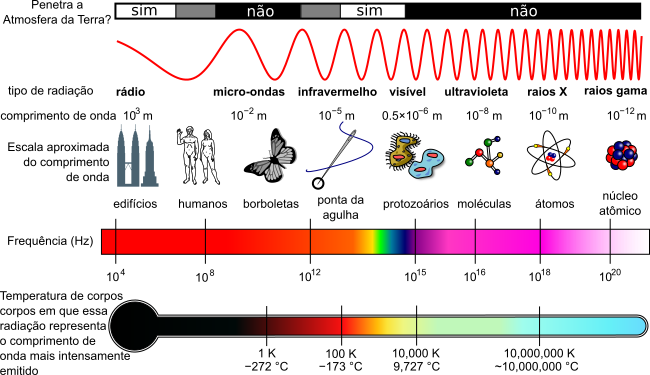
\includegraphics[width=\linewidth]{img/espectro.png}
	\caption{Espectro eletromagnético.}
	\label{fig:esel}
	\centering
\end{figure}

O olho humano tem capacidade de enxergar apenas uma pequena parte do espectro
eletromagnético.

% ---
% Finaliza a parte no bookmark do PDF, para que se inicie o bookmark na raiz
% ---
\bookmarksetup{startatroot}% 
% ---

% ---
% Conclusão
% ---
\section{Considerações finais}
\addcontentsline{toc}{section}{Considerações finais}

\lipsum[1]

\begin{citacao}
\lipsum[2]
\end{citacao}

\lipsum[3]
\newpage
% ----------------------------------------------------------
% ELEMENTOS PÓS-TEXTUAIS
% ----------------------------------------------------------
\postextual{}

% ----------------------------------------------------------
% Referências bibliográficas
% ----------------------------------------------------------
\bibliography{abntex2-modelo-references}


\end{document}
